\documentclass[12pt]{article}
\usepackage{amsmath}
\usepackage{array}
\usepackage{graphicx}
\usepackage{indentfirst}
\usepackage{listings}
\usepackage{xcolor}
\usepackage{fontspec}
\usepackage{multirow}
\usepackage{ctex}
\usepackage{ulem}
\usepackage{float}
\usepackage{tabularx}
\usepackage{geometry}
\usepackage{longtable}
\usepackage{setspace}
\usepackage{amssymb}
% \geometry{
%     left=3cm,
%     right=3cm,
%     top=3cm,
%     bottom=3cm,
%     % 如果需要设置页眉页脚的高度，可以添加以下参数
%     % headheight=2cm,
%     % headsep=1cm,
%     % footskip=1cm,
% }
\renewcommand{\arraystretch}{1.3} %控制行高

\begin{document}

\begin{titlepage}
    \centering
    
    
\includegraphics[width=0.6\textwidth]{./picture/logo.jpg}\\[1.5cm]
    
    % 标题
    {\LARGE \textbf{本科实验报告}}\\[4cm]

    \begin{large}
        \makebox[4em][s]{课程名称}:\underline{\makebox[15em][c]{B/S体系软件设计}}\\[0.5cm]
        \makebox[4em][s]{姓名}:\underline{\makebox[15em][c]{李谞远}}\\[0.5cm]
        \makebox[4em][s]{学院}:\underline{\makebox[15em][c]{计算机科学与技术学院}}\\[0.5cm]
        \makebox[4em][s]{院系}:\underline{\makebox[15em][c]{计算机系}}\\[0.5cm]
        \makebox[4em][s]{专业}:\underline{\makebox[15em][c]{软件工程}}\\[0.5cm]
        \makebox[4em][s]{学号}:\underline{\makebox[15em][c]{3220102970}}\\[0.5cm]
        \makebox[4em][s]{指导教师}:\underline{\makebox[15em][c]{胡晓军}}\\[1cm]
    \end{large}

    {\Large \textbf{\today}}

\end{titlepage}

\newpage
\begin{center}
  \zihao{3} \bf 浙江大学实验报告
  \end{center}
  \vspace{1cm}
  \zihao{-4}
  \noindent 课程名称: \underline{\makebox[5cm]{B/S体系软件设计}} 
  \\[0.4cm] 
  实验项目名称: \underline{\makebox[11.3cm]{商品价格比较网站}} \\[0.4cm] 
  学生姓名: \underline{\makebox[2cm]{李谞远}} 
  专业: \underline{\makebox[4.6cm]{软件工程}} 
  学号: \underline{\makebox[3cm]{3220102970}} \\[0.4cm]
  同组学生姓名: \underline{\makebox[4.2cm]{无}} 
  指导老师: \underline{\makebox[5cm]{胡晓军}} \\[0.4cm]
  实验地点: \underline{\makebox[5cm]{无}}
  实验日期: \underline{\makebox[1.4cm]{2024}} 年 \underline{\makebox[0.9cm]{11}} 月 \underline{\makebox[0.9cm]{5}} 日
\newpage  
\tableofcontents
\newpage

\section{设计概述}

\subsection{任务和目标}
本项目旨在开发一个商品价格比较网站，使用户能够通过该平台比较不同电商平台上的商品价格。该网站需提供用户注册、登录功能，支持至少两个主流电商平台的商品价格查询，建立商品库以存储商品信息和价格，并提供商品查询界面。此外，网站应支持设置降价提醒，并确保界面适配手机，以提供良好的移动端用户体验。

\subsection{需求概述}

\subsubsection{功能需求}
需要实现的基本功能如下：

\begin{enumerate}
    \item 实现用户注册、登录功能，用户注册时需要填写必要的信息并验证，如用户名、密码要求在6字节以上，email的格式验证，并保证用户名和email在系统中唯一，用户登录后可以进行以下操作。
    \item 通过商品名称在主流电商平台上查询该商品实时价格
    \item 支持至少2个以上平台查询价格进行比较（淘宝、京东等）
    \begin{itemize}
        \item 商品名称建议分词处理优化查询；
        \item 查询多个结果的处理；
        \item 很多平台需要平台用户登录验证后才可以进行查询。
    \end{itemize}
    \item 建立商品库，将商品信息和商品价格保存在数据库中。商品信息包含名称、多级品类、规格、条码、图片等，方便后续查询。
    \item 提供商品查询界面能显示商品信息，把历史价格用图表形式显示（如价格走势图）。
    \item 支持设置降价提醒，针对指定商品定时查询最新价格，如有降价发送提醒，可以通过邮件，App推送等方式实现。
    \item 样式适配手机，开发手机App或能够在手机浏览器/微信等应用内置的浏览器中友好显示。
    \item 如开发手机端，可以用相机拍摄商品图片或扫码商品条码进行商品查询。
\end{enumerate}

\subsubsection{性能需求}
\begin{itemize}
    \item 用户注册和登录响应时间不超过3秒。
    \item 商品查询响应时间不超过5秒，包括从电商平台获取数据和数据库查询。
    \item 系统应能支持至少500个并发用户。
    \item 服务器配置要求：
        \begin{itemize}
            \item 至少4核CPU，8GB RAM。
            \item SSD硬盘，至少256GB存储空间。
            \item 支持HTTPS协议的Web服务器。
        \end{itemize}
    \item 数据库应能处理至少10万条商品记录，响应时间不超过2秒。
\end{itemize}

\subsubsection{安全性需求}
\begin{itemize}
    \item \textbf{数据加密：} 所有敏感数据，主要是用户信息和配置信息等，必须在存储和传输过程中进行加密。使用加密算法（如AES-256）进行数据加密。
    \item \textbf{安全通信：} 使用HTTPS协议进行所有网络通信，确保数据传输的安全性。
    \item \textbf{输入验证：} 对所有用户输入进行严格的验证，防止SQL注入、XSS攻击和其他常见的注入攻击。使用白名单输入验证策略。
    \item \textbf{错误处理：} 设计健壮的错误处理机制，避免向用户泄露敏感的系统信息。所有错误消息应对外部用户隐藏内部细节，只提供有用的信息。
    \item \textbf{安全配置：} 确保所有系统组件（如服务器、数据库、应用程序）都按照安全配置指南进行配置，关闭不必要的服务和端口，限制对关键资源的访问。
\end{itemize}

\subsubsection{可维护性需求}
\begin{itemize}
    \item \textbf{模块化设计：} 系统应采用模块化设计，实现高内聚、低耦合的系统模块划分。这种设计有利于提高模块的独立性，使得在修改或扩展功能时对其他模块的影响最小。
    \item \textbf{文档完整性：} 提供完备、清晰、可读的文档，包括设计文档、用户手册、API文档等，以提高系统的可读性和可修改性。文档应具有简明性和书写风格的一致性，方便操作人员快速查阅及维护人员系统掌握。
    \item \textbf{编程规范：} 代码应遵循良好的编程风格，包括详细的注释、统一的编程格式、清晰的结构和明确的注释，以便调试和测试人员能快速定位错误。避免使用模糊不清的代码，使用有意义的变量和函数命名，以及适当的、格式正确的注释。
    \item \textbf{单元测试：} 对核心模块编写单元测试，确保各子模块和系统整体的正常运作。测试应具有模块化和良好的结构，能够显示任意的中间结果，并以清楚的描述方式说明系统的输出。
    \item \textbf{性能监控：} 实时监控系统的性能指标，及时发现和解决性能瓶颈，确保系统能够快速响应用户请求。性能监控应包括但不限于响应时间、系统负载、资源使用情况等。
\end{itemize}

\section{总体设计}

\subsection{基本设计概念}
本项目的总体设计遵循模块化和分层的原则，以确保系统的可扩展性、可维护性和可重用性。系统将分为以下几个主要模块：
\begin{itemize}
    \item 用户管理模块：负责用户注册、登录、信息管理等功能。
    \item 商品查询模块：实现商品信息的查询和价格比较功能。
    \item 数据库管理模块：负责商品信息和价格数据的存储和管理。
    \item 价格监控模块：提供降价提醒和价格变化跟踪功能。
    \item 前端展示模块：提供用户界面，包括商品查询界面和历史价格图表展示。
    \item 移动端适配模块：确保网站在移动设备上的良好显示和用户体验。
\end{itemize}

系统的开发将采用前后端分离的架构，前端使用Vue.js框架，后端使用Spring Boot框架，数据库采用MySQL，爬虫使用Python实现。前端发送HTTP请求到后端，后端处理请求并返回数据，前端负责展示数据和用户交互。

\subsection{技术栈}

\subsubsection{前端}
\begin{itemize}
    \item 技术：HTML、CSS、JavaScript
    \item 框架：Vue.js
\end{itemize}

\subsubsection{后端}
\begin{itemize}
    \item 语言：Java
    \item 框架：Spring Boot
    \item 数据库：MySQL
    \item 爬虫：Python
\end{itemize}

\subsubsection{客户端}
支持主流浏览器，如Chrome、Firefox、Edge等，手机端适配iOS和Android系统。

\subsection{技术介绍}
下面对系统中使用的主要技术进行简要介绍。
\subsubsection{前端}
\begin{itemize}
    \item \textbf{HTML}：超文本标记语言（HTML）是构建网页内容的标准标记语言，用于定义网页的结构和内容。
    \item \textbf{CSS}：层叠样式表（CSS）是一种样式表语言，用于设置HTML文档的样式，包括布局、颜色和字体。
    \item \textbf{JavaScript}：JavaScript是一种高级的、解释型的编程语言，主要用于网页上实现动态效果和用户交互。
    \item \textbf{Vue.js}：Vue.js是一个渐进式JavaScript框架，用于构建用户界面，它提供了响应式数据绑定和组件化，使得开发单页应用（SPA）变得简单。
\end{itemize}

\subsubsection{后端}
\begin{itemize}
    \item \textbf{Java}：Java是一种广泛使用的高级编程语言，具有跨平台、面向对象和高安全性等特点，适用于企业级应用开发。
    \item \textbf{Spring Boot}：Spring Boot是基于Spring框架的项目，它简化了基于Spring的应用程序的初始搭建以及开发过程，可以创建独立、生产级的基于Spring框架的应用程序。
    \item \textbf{MySQL}：MySQL是一个流行的关系型数据库管理系统，它提供了多用户和多线程的数据存储、查询和管理功能。
    \item \textbf{Python}：Python是一种高级、解释型、通用的编程语言，它具有清晰的语法和结构，广泛用于Web开发、科学计算和自动化脚本编写。
\end{itemize}

\subsubsection{版本控制}
\begin{itemize}
    \item \textbf{Git}：Git是一个分布式版本控制系统，它允许开发人员跟踪文件和目录的更改，支持多人协作开发，是现代软件开发中不可或缺的工具。
\end{itemize}

\subsubsection{容器化}
\begin{itemize}
    \item \textbf{Docker}：Docker是一个开源的应用容器引擎，它允许开发者将应用及其依赖打包在一起来创建可移植的容器，从而实现快速部署和迁移。
    \item \textbf{Docker Compose}：Docker Compose是一个用于定义和运行多容器Docker应用的工具，通过一个YAML文件进行配置，然后使用一个命令来创建和启动所有服务，简化了容器化应用的管理。
\end{itemize}

\section{接口设计}
% 用户注册接口
\subsection{用户注册接口}
\begin{longtable}{|p{3cm}|p{10cm}|}
\hline
\textbf{URL} & /api/register \\ \hline
\textbf{请求方式} & POST \\ \hline
\textbf{请求体} &
\begin{verbatim}
{
  "username": "string",
  "password": "string",
  "email": "string"
}
\end{verbatim} \\ \hline
\textbf{返回值} &
\begin{verbatim}
{
  "status": "success",
  "message": "User registered successfully"
}
\end{verbatim} \\ \hline
\textbf{作用简介} & 此接口用于用户注册，接收用户名、密码和电子邮件地址，并验证这些信息的有效性，需要确保用户名和电子邮件在系统中唯一。 \\ \hline
\end{longtable}

% 用户登录接口
\subsection{用户登录接口}
\begin{longtable}{|p{3cm}|p{10cm}|}
\hline
\textbf{URL} & /api/login \\ \hline
\textbf{请求方式} & POST \\ \hline
\textbf{请求体} &
\begin{verbatim}
{
  "username": "string",
  "password": "string"
}
\end{verbatim} \\ \hline
\textbf{返回值} &
\begin{verbatim}
{
  "status": "success",
  "token": "JWT Token"
}
\end{verbatim} \\ \hline
\textbf{作用简介} & 此接口用于用户登录，验证用户名和密码，如果验证成功，返回一个JWT（JSON Web Token）用于后续的认证。 \\ \hline
\end{longtable}

% 商品查询接口
\subsection{商品查询接口}
\begin{longtable}{|p{3cm}|p{10cm}|}
\hline
\textbf{URL} & /api/search \\ \hline
\textbf{请求方式} & POST \\ \hline
\textbf{请求体} &
\begin{verbatim}
{
  "name": "string"
}
\end{verbatim} \\ \hline
\textbf{返回值} &
\begin{verbatim}
{
  "status": "success",
  "data": [
    {
      "id": "integer",
      "name": "string",
      "price": "float",
      "platform": "string",
      "image_url": "string"
    }
  ]
}
\end{verbatim} \\ \hline
\textbf{作用简介} & 此接口用于根据商品名称查询多个电商平台上的商品实时价格，返回包含匹配商品的结果列表。支持分词处理优化查询。 \\ \hline
\end{longtable}

% 降价提醒设置接口
\subsection{降价提醒设置接口}
\begin{longtable}{|p{3cm}|p{10cm}|}
\hline
\textbf{URL} & /api/price-alerts \\ \hline
\textbf{请求方式} & POST \\ \hline
\textbf{请求体} &
\begin{verbatim}
{
  "user_id": "integer",
  "product_id": "integer",
  "original_price": "float",
  "current_price": "float",
}
\end{verbatim} \\ \hline
\textbf{返回值} &
\begin{verbatim}
{
  "status": "success",
  "message": "Price alert set successfully"
}
\end{verbatim} \\ \hline
\textbf{作用简介} & 此接口用于用户设置降价提醒，当商品价格低于用户设定的目标价格时，系统将通过邮件或App推送等方式发送提醒。 \\ \hline
\end{longtable}

% 商品信息获取接口
\subsection{商品信息获取接口}
\begin{longtable}{|p{3cm}|p{10cm}|}
\hline
\textbf{URL} & /api/products/{id} \\ \hline
\textbf{请求方式} & POST \\ \hline
\textbf{请求体} & 无 \\ \hline
\textbf{返回值} &
\begin{verbatim}
{
  "status": "success",
  "data": {
    "id": "integer",
    "name": "string",
    "category": "string",
    "specification": "string",
    "barcode": "string",
    "image_url": "string",
    "price_history": [
      {
        "date": "date",
        "price": "float"
      }
    ]
  }
}
\end{verbatim} \\ \hline
\textbf{作用简介} & 此接口用于获取特定商品的详细信息，包括名称、类别、规格、条码、图片以及历史价格图表数据。 \\ \hline
\end{longtable}

% 商品价格历史接口
\subsection{商品价格历史接口}
\begin{longtable}{|p{3cm}|p{10cm}|}
  \hline
  \textbf{URL} & /api/history/{id} \\ \hline
  \textbf{请求方式} & POST \\ \hline
  \textbf{请求体} & 无 \\ \hline
  \textbf{返回值} &
  \begin{verbatim}
  {
    "status": "success",
    "data": {
      "id": "integer",
      "name": "string",
      "price_history": [
        {
          "date": "date",
          "price": "float"
        }
      ]
    }
  }
  \end{verbatim} \\ \hline
  \textbf{作用简介} & 此接口用于获取特定商品的历史价格数据，返回包含商品名称和历史价格数据的结果，用于制作图表。 \\ \hline
  \end{longtable}

\section{用户界面}
下面制作了一些用户界面的原型设计，包括用户注册界面、用户登录界面、商品查询界面和商品比价界面，以手机端为例。

\subsection{用户注册界面}
\begin{figure}[H]
    \centering
    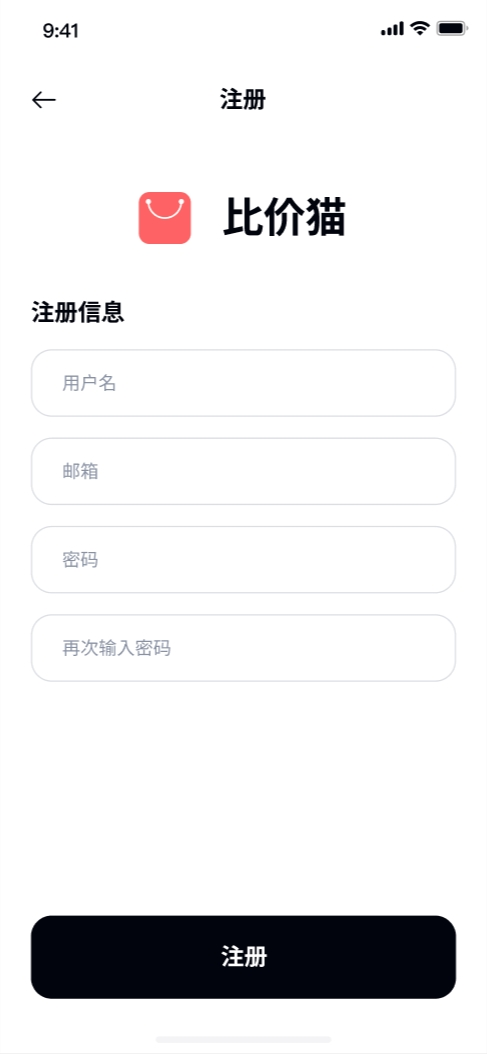
\includegraphics[width=0.5\textwidth]{./picture/注册.png}
    \caption{用户注册界面}
\end{figure}

\subsection{用户登录界面}
\begin{figure}[H]
  \centering
  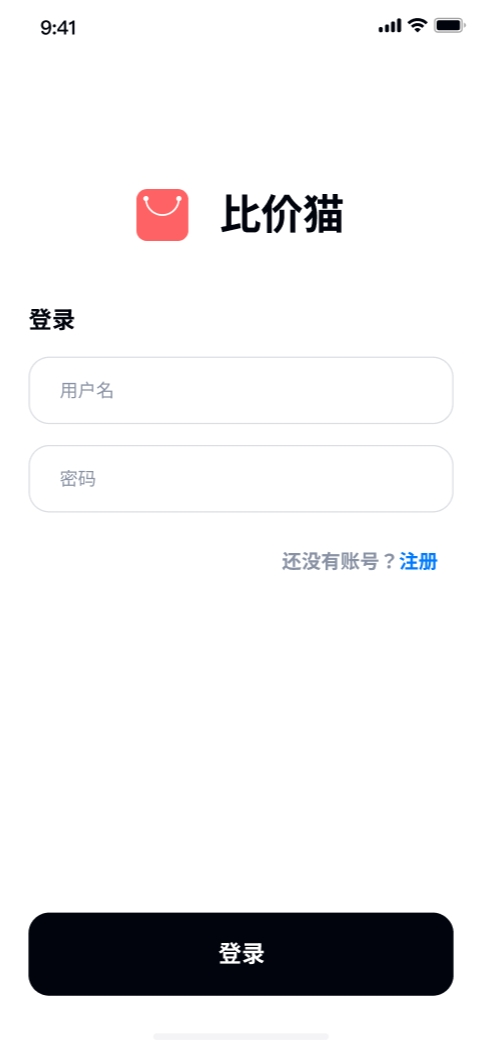
\includegraphics[width=0.5\textwidth]{./picture/登录.png}
  \caption{用户登录界面}
\end{figure}

\subsection{商品查询界面}
\begin{figure}[H]
  \centering
  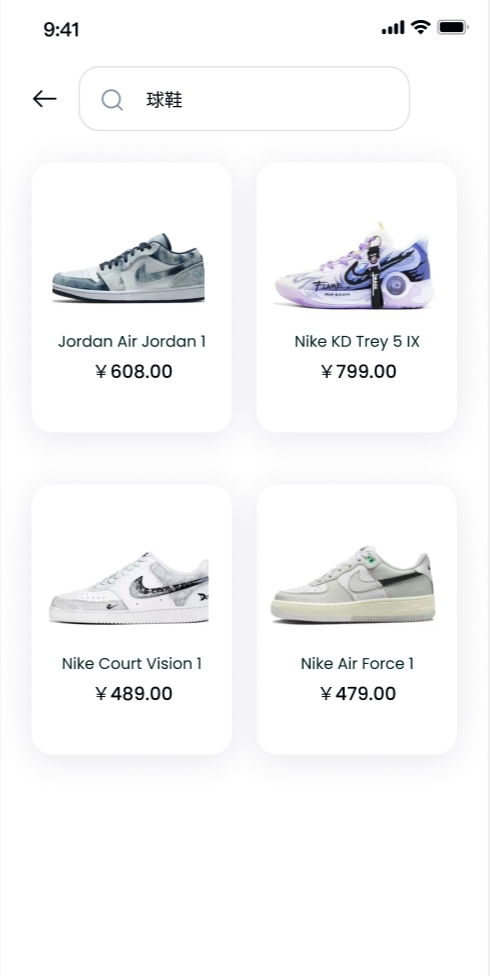
\includegraphics[width=0.5\textwidth]{./picture/商品查询.png}
  \caption{商品查询界面}
\end{figure}

\subsection{商品比价界面}
\begin{figure}[H]
  \centering
  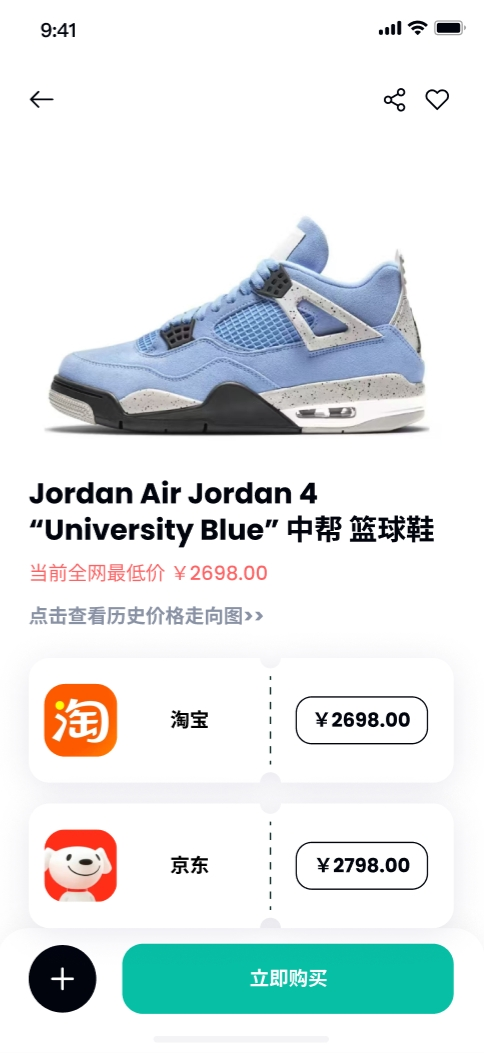
\includegraphics[width=0.5\textwidth]{./picture/商品比价.png}
  \caption{商品比价界面}
\end{figure}

\section{数据库设计}

\subsection{概念结构设计}
本项目的数据库需要满足以下要求：
\begin{itemize}
    \item 存储用户信息（用户名、密码、邮箱等）。
    \item 存储商品信息（名称、分类、规格、条码、图片、价格等）。
    \item 存储价格历史数据，用于绘制价格走势。
    \item 存储用户的搜索历史，记录用户查询的商品名称及时间。
\end{itemize}
基于需求，E-R 图的核心实体和关系包括：
\begin{itemize}
    \item 用户（User）
    \item 商品（Product）
    \item 商品价格历史（PriceHistory）
    \item 搜索历史（SearchHistory）
\end{itemize}

\subsection{逻辑结构设计}
数据库表结构设计如下：

\begin{longtable}{|p{3cm}|p{4cm}|p{8cm}|}
\hline
\textbf{表名} & \textbf{字段名} & \textbf{描述} \\ \hline

User & id (PK) & 用户唯一标识 \\ \cline{2-3}
& username & 用户名，要求唯一 \\ \cline{2-3}
& password & 密码 \\ \cline{2-3}
& email & 邮箱地址，要求唯一 \\ \hline

Product & id (PK) & 商品唯一标识 \\ \cline{2-3}
& name & 商品名称 \\ \cline{2-3}
& category & 商品分类（多级品类） \\ \cline{2-3}
& specification & 商品规格描述 \\ \cline{2-3}
& barcode & 商品条码 \\ \cline{2-3}
& image\_url & 商品图片链接 \\ \hline

PriceHistory & id (PK) & 唯一标识 \\ \cline{2-3}
& product\_id (FK) & 商品唯一标识 \\ \cline{2-3}
& date & 记录日期 \\ \cline{2-3}
& price & 当日价格 \\ \hline

SearchHistory & id (PK) & 唯一标识 \\ \cline{2-3}
& user\_id (FK) & 用户唯一标识 \\ \cline{2-3}
& search\_term & 搜索关键词 \\ \cline{2-3}
& search\_date & 搜索日期 \\ \hline

\end{longtable}

\subsection{物理结构设计}
\begin{itemize}
    \item 数据库名称：\texttt{PriceComparisonDB}
    \item 存储引擎：MySQL 默认 InnoDB，支持事务和外键。
    \item 索引设计：
    \begin{itemize}
        \item \texttt{User.username} 和 \texttt{User.email} 设置唯一索引。
        \item \texttt{PriceHistory.product\_id} 和 \texttt{SearchHistory.user\_id} 添加外键索引。
    \end{itemize}
\end{itemize}
以下为数据库创建的 SQL 脚本：

\begin{verbatim}
CREATE DATABASE PriceComparisonDB;

USE PriceComparisonDB;

CREATE TABLE User (
    id INT AUTO_INCREMENT PRIMARY KEY,
    username VARCHAR(255) UNIQUE NOT NULL,
    password VARCHAR(255) NOT NULL,
    email VARCHAR(255) UNIQUE NOT NULL
);

CREATE TABLE Product (
    id INT AUTO_INCREMENT PRIMARY KEY,
    name VARCHAR(255) NOT NULL,
    category VARCHAR(255),
    specification TEXT,
    barcode VARCHAR(255),
    image_url TEXT
);

CREATE TABLE PriceHistory (
    id INT AUTO_INCREMENT PRIMARY KEY,
    product_id INT NOT NULL,
    date DATE NOT NULL,
    price FLOAT NOT NULL,
    FOREIGN KEY (product_id) REFERENCES Product(id)
);

CREATE TABLE SearchHistory (
    id INT AUTO_INCREMENT PRIMARY KEY,
    user_id INT NOT NULL,
    search_term VARCHAR(255) NOT NULL,
    search_date DATE NOT NULL,
    FOREIGN KEY (user_id) REFERENCES User(id)
);
\end{verbatim}

\subsection{ER图}
\begin{figure}[H]
    \centering
    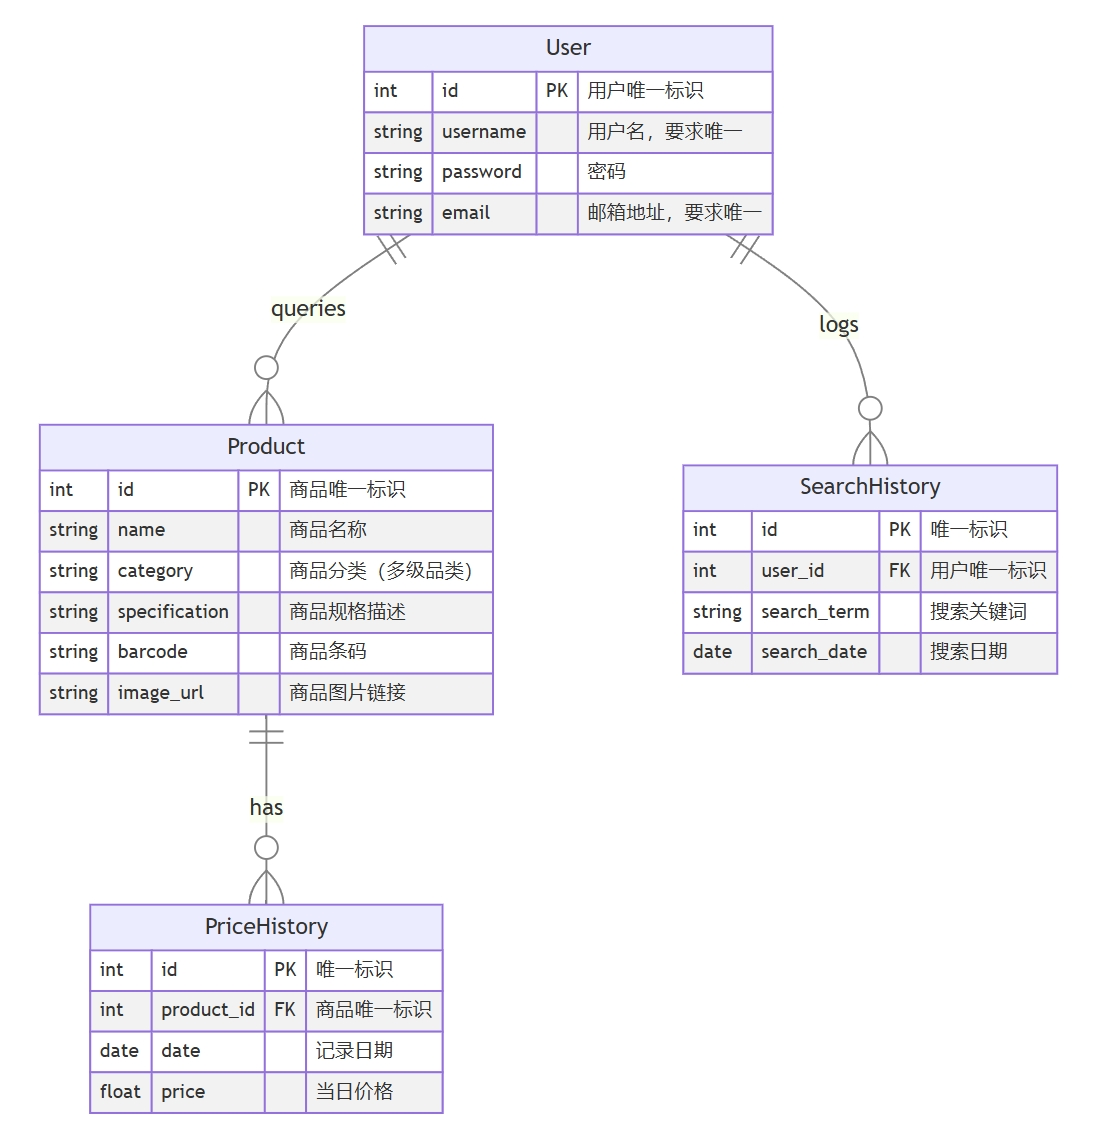
\includegraphics[width=0.8\textwidth]{./picture/ER.png}
    \caption{数据库ER图}
\end{figure}

\section{系统出错设计}

\subsection{出错信息}
出错信息是系统在运行过程中遇到问题时向用户或管理员提供的反馈。以下是一些常见的出错信息及其含义：

\begin{table}[H]
    \centering
    \begin{tabular}{|m{5cm}<{\centering}|m{3.5cm}<{\centering}|m{6cm}<{\centering}|}
    \hline
    \textbf{系统输出} & \textbf{含义} & \textbf{解决方法} \\ \hline
    404 Not Found & 请求的资源未找到 & 检查URL是否正确，或联系管理员确认资源是否存在 \\ \hline
    500 Internal Server Error & 服务器内部错误 & 服务器可能遇到未知的错误，需要管理员检查服务器日志 \\ \hline
    Database Connection Error & 数据库连接失败 & 检查数据库服务是否运行，网络连接是否正常 \\ \hline
    Invalid User Input & 用户输入无效 & 提示用户重新输入有效数据 \\ \hline
    Timeout Error & 请求超时 & 增加请求超时时间，或检查网络连接 \\ \hline
    Authentication Failed & 认证失败 & 检查用户名和密码是否正确，或重置密码 \\ \hline
    \end{tabular}
\end{table}

\subsection{补救措施}
\subsubsection{系统恢复}
在发生故障后，根据系统日志，将系统恢复到正常运行状态。通常包括重启服务、恢复备份等操作。

\subsubsection{数据恢复}
在数据丢失或损坏后，根据定期备份的数据，将数据恢复到正常状态。如果是代码损坏，利用Github等版本控制工具，恢复代码到最近的可用版本。

\subsubsection{人工处理}
在系统自动恢复措施无效时，由管理员介入处理，包括检查日志、修复代码错误、更新配置等。

\subsection{系统维护设计}
为了确保系统的稳定运行和安全性，以下是一些关键的系统维护策略：

\begin{itemize}
    \item \textbf{操作审计}：系统应记录所有用户操作的详细日志，包括操作时间、操作类型和操作结果，以便于事后审计和追踪可能的安全问题。
    \item \textbf{安全漏洞管理}：系统维护人员应定期检查和更新系统，修补已知的安全漏洞，以防止潜在的攻击。
    \item \textbf{数据库完整性检查}：定期对数据库进行完整性检查，包括数据备份、恢复测试和性能优化，确保数据的完整性和可用性。
    \item \textbf{异常处理机制}：在系统的关键部分实现异常处理机制，使用try-catch语句捕获异常，并记录详细的错误信息，以便快速定位和解决问题。
    \item \textbf{性能监控}：实施实时性能监控，定期分析系统性能指标，如响应时间、资源使用情况等，及时发现并解决性能瓶颈。
    \item \textbf{代码质量保证}：采用代码审查和静态代码分析工具，确保代码质量，减少潜在的错误和安全风险。
\end{itemize}

\end{document}